\input{preamble}
\begin{center}
{\LARGE Eigenmath Manual}

\bigskip
9634295@gmail.com
\end{center}

\begin{center}
\begin{tikzpicture}
\node at (0,0) {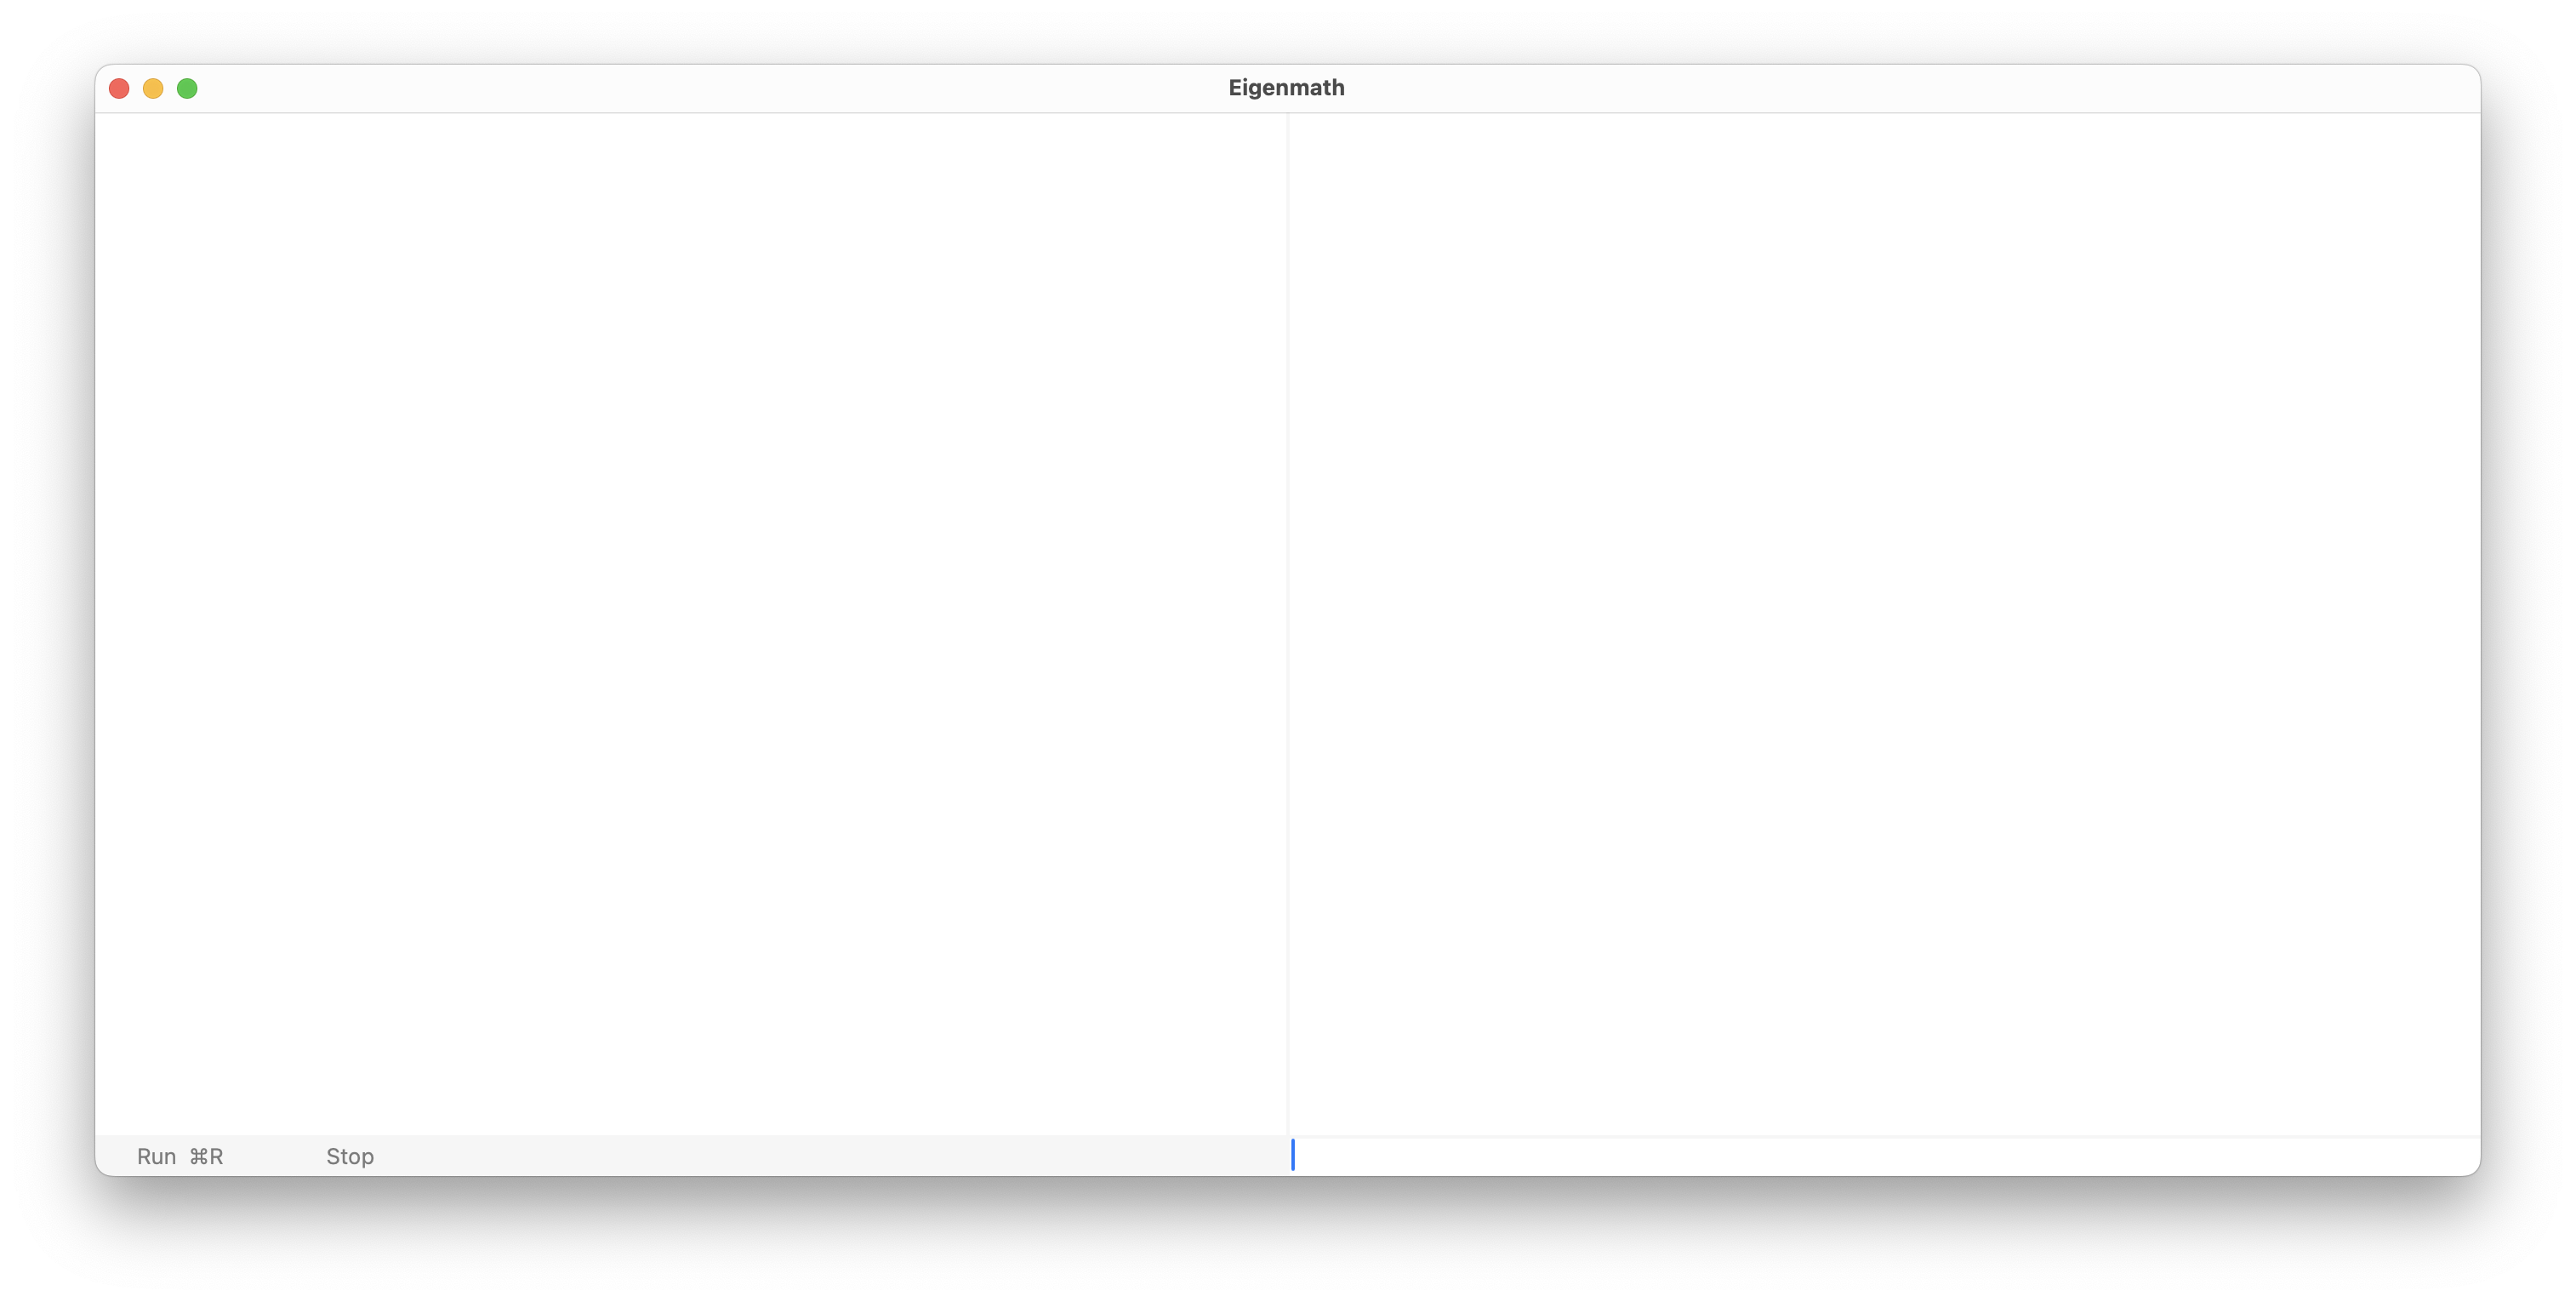
\includegraphics[scale=0.3]{screenshot.png}};
\draw (-4,2) node {Scripts go here};
\draw (4,2) node {Results appear here};
\draw (3.6,-4) node {Commands are entered here};
\draw (3.8,-3.5) node {$\uparrow$};
\end{tikzpicture}
\end{center}

Multiple commands can be put together in a script.
Scripts are run by clicking the Run button.
After a script runs, all of the results are available in command mode.
To export a result, click on the result text.
The result can now be printed or copied to the pasteboard.
(Note that it is necessary to click on the result text
instead of somewhere else in the result window.)

\iffalse
\bigskip
To print or copy results, click in the result field.
Then press \cmd$\,$P to print, \cmd$\,$C to copy to the clipboard.
\fi

\bigskip
Note: Times New Roman and Times New Roman Italic fonts need
to be the standard Mac fonts that include special symbols and Greek letters.
See the following link for correcting font problems.

\bigskip
{\footnotesize\verb$support.apple.com/guide/font-book/restore-fonts-that-came-with-your-mac-fb34862/mac$}

\newpage
\tableofcontents

\end{document}
